\documentclass[11pt, oneside]{article}  
\usepackage[margin=0.5in]{geometry} % Margins
\usepackage[ampersand]{easylist} % Bullets for lists
\usepackage[bottom]{footmisc}  % Glue footnotes to bottom
\usepackage{graphicx}
\graphicspath{ {imgs/} }

\title{Operating Systems Principles\\UCLA-CS111-W18}
\author{Quentin Truong\\Taught by Professor Reiher}
\date{Winter 2018}


\begin{document}
\maketitle
\tableofcontents
\pagenumbering{arabic}
\clearpage


%========================================================
\section{L3: Arpaci-Dusseau Chapter 5: Interlude: Process API}
\subsection{The fork() System Call}
	\begin{easylist}  
	\ListProperties(Hide=100, Hang=true, Progressive=4ex, Style*=--\ , Style2*=$\bullet\ $)
        & Crux: How to create and control processes
		& fork()
        && Creates new process; returns child's PID to parent; returns 0 to child;
        && Each has own PC, registers, address space
        & Nondeterministic Behavior
        && Scheduler will decide which process to run
        && May lead to problems in multi-threaded programs
	\end{easylist}

\subsection{The wait() System Call}
    \begin{easylist}  
    \ListProperties(Hide=100, Hang=true, Progressive=4ex, Style*=--\ , Style2*=$\bullet\ $)
        & wait()
        && Parent calls wait() to wait for child to finish execution
    \end{easylist}

\subsection{The exec() System Call}
    \begin{easylist}  
    \ListProperties(Hide=100, Hang=true, Progressive=4ex, Style*=--\ , Style2*=$\bullet\ $)
        & exec()
        && Loads code, overwrites code segment, and reinitializes memory space
        && Takes exceutable name and arguments
        && Does not create a new process; transform current process
    \end{easylist}

\subsection{Why? Motivating The API}
    \begin{easylist}  
    \ListProperties(Hide=100, Hang=true, Progressive=4ex, Style*=--\ , Style2*=$\bullet\ $)
        & Separation
        && Separating fork() and exec() allows code to alter the environment of the about-to-run program
        & Example
        && Shell forks a process, execs the program, and waits until finished
        && The separation allows for things such as output to be redirected (closes stdout and opens file)
    \end{easylist}

\subsection{Other Parts Of The API}
    \begin{easylist}  
    \ListProperties(Hide=100, Hang=true, Progressive=4ex, Style*=--\ , Style2*=$\bullet\ $)
        & kill()
        && System call sends signal to process to sleep, die, etc
    \end{easylist}
%========================================================

%========================================================
\section{L3: Arpaci-Dusseau Chapter 6: Mechanism: Limited Direct Execution}
\subsection{Basic Technique: Limited Direct Execution}
    \begin{easylist}  
    \ListProperties(Hide=100, Hang=true, Progressive=4ex, Style*=--\ , Style2*=$\bullet\ $)
        & Crux: How to efficiently virtualize CPU with control
        & Limited Direct Execution
        && OS will create entry for process list, allocate memory for program, load program into memory, setup stack with argc/v, clear registers, execute call to main()
        && Program will run main(), execute return
        && OS will free memory, remove from process list
        & LDE good bc fast, but
        && Problem of keeping control
        && Problem of time sharing still
    \end{easylist}

\subsection{Problem 1: Restricted Operations}
    \begin{easylist}  
    \ListProperties(Hide=100, Hang=true, Progressive=4ex, Style*=--\ , Style2*=$\bullet\ $)
        & User mode vs. Kernel mode
        && Restricted mode which needs to ask kernel to perform system calls
        && Calls like open() are actually procedure calls with trap to enter kernel and raise privilege
        && Return-from-trap is used to enter user mode from kernel and drop privilege
        && Push counters, flags, registers onto per-process kernel stack when trapping
        & Trap table is used to control what code is executed when trapping
        && Trap handler used by hardware to cause interrupts 
        && Telling hardware where trap table is is privileged
        && Trap handler actually uses system-call number, rather than specifying an address (another layer of protection)
        & Two phases of LDE
        && At boot, kernel initializes trap table and remembers where it is
        \begin{figure}[h]
            \centering
            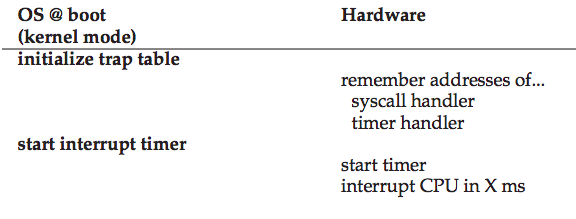
\includegraphics[scale=0.6]{boot}
        \end{figure}
    \end{easylist}

\subsection{Problem 2: Switching Between Processes}
    \begin{easylist}  
    \ListProperties(Hide=100, Hang=true, Progressive=4ex, Style*=--\ , Style2*=$\bullet\ $)
        & How can OS regain control?
        && Because process is running, so OS is not running
        & Cooperative Approach
        && System calls include explicit yield system call, transfering control back to OS
        & Noncooperative Approach
        && Reboot, Timer Interrupt
        & Saving and Restoring Context
        && Scheduler will choose when to switch processes
    \end{easylist}
    \begin{figure}[h]
        \centering
        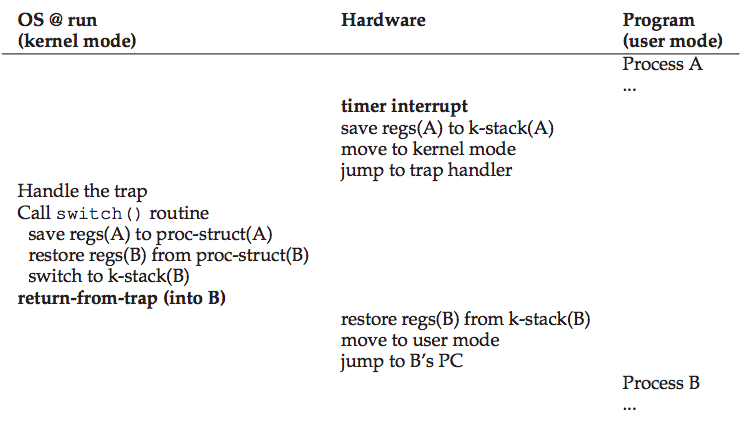
\includegraphics[scale=0.5]{context_switch}
    \end{figure}

\subsection{Worried About Concurrency?}
    \begin{easylist}  
    \ListProperties(Hide=100, Hang=true, Progressive=4ex, Style*=--\ , Style2*=$\bullet\ $)
        & Interrupt during interrupt?
        && Many complex things to do
        && Could disable interrupts (but this might lose interrupts), or locking schemes, etc
    \end{easylist}

\subsection{Summary}
    \begin{easylist}  
    \ListProperties(Hide=100, Hang=true, Progressive=4ex, Style*=--\ , Style2*=$\bullet\ $)
        & Reboot
        && Good technique because restores system to well-tested state
        && OS will 'baby-proof' by only allowing processes to run in restricted mode and with interrupt handlers
    \end{easylist}
%========================================================

%========================================================
\section{L3: Linking and Libraries: Object Modules, Linkage Editing, Libraries}
\subsection{Introduction}
    \begin{easylist}  
    \ListProperties(Hide=100, Hang=true, Progressive=4ex, Style*=--\ , Style2*=$\bullet\ $)
        & Process as fundamental; as executing instance of program
        && Program as one or more files (these are not the executables though)
        && Source must be translated
    \end{easylist}

\subsection{The Software Generation Tool Chain}
    \begin{easylist}  
    \ListProperties(Hide=100, Hang=true, Progressive=4ex, Style*=--\ , Style2*=$\bullet\ $)
        & Source module
        && Editable text in some language like C
        & Relocatable object module
        && Sets of compiled instructions; incomplete programs
        & Library
        && Collection of object modules
        & Load module
        && Complete programs ready to be loaded into memory
        & Compiler
        && Parse source modules; usually generates assembly, may generate pseudo-machine
        & Assembler
        && Object module with mostly machine code
        && Memory addresses of functions, variables may not be filled in
        & Linkage Editor
        && Find all required object modules and resolve all references
        & Program Loader
        && Examines load module, creates virtual space, reads instructions, initializes data values
        && Find and map additional shared libraries
    \end{easylist}

\subsection{Object Modules}
    \begin{easylist}  
    \ListProperties(Hide=100, Hang=true, Progressive=4ex, Style*=--\ , Style2*=$\bullet\ $)
        & Code in multiple files
        && Because more understandable if splitting functionality
        && Many functions are reused, so use external libraries
        & Relocatable object modules are program fragments
        && Incomplete because make references to code in other modules
        && Even the references to other code are only relative 
        & ELF format
        && Header section with types, sizes, and location of other sections
        && Code and data section to be loaded contiguously
        && Symbol table of external symbols
        && Relocation entries describing location of field, width/type of field, symbol table entry
    \end{easylist}

\subsection{Libraries}
    \begin{easylist}  
    \ListProperties(Hide=100, Hang=true, Progressive=4ex, Style*=--\ , Style2*=$\bullet\ $)
        & Reusable, standard functions in libraries 
        && Libraries not always orthogonal and independent
        & Build program by combining object modules and resolving external references 
    \end{easylist}

\subsection{Linkage Editing}
    \begin{easylist}  
    \ListProperties(Hide=100, Hang=true, Progressive=4ex, Style*=--\ , Style2*=$\bullet\ $)
        & Resolution
        && Search libraries to find object modules to resolve external references
        & Loading
        && Lay text and data in single virtual address space
        & Relocation
        && Ensure references correctly reflect chosen address
    \end{easylist}

\subsection{Load Modules}
    \begin{easylist}  
    \ListProperties(Hide=100, Hang=true, Progressive=4ex, Style*=--\ , Style2*=$\bullet\ $)
        & Load module requires no relocation and is complete
        & When loading new module
        && Determine required text and data sizes and locations, allocate segments, read contents, create a stack segment with pointer
        & Load module has symbol table to help determine where exceptions occurred
    \end{easylist}

\subsection{Static vs. Shared Libraries}
    \begin{easylist}  
    \ListProperties(Hide=100, Hang=true, Progressive=4ex, Style*=--\ , Style2*=$\bullet\ $)
        & Static Linking
        && Many copies, so inefficient; also, permenant copy, so don't receive updates
        & Shared Libraries
        && Implementations vary, but one way
        &&& Reserve address for libraries, linkage edit, map with redirection table, etc, more mapping
        && Efficient, but doesn't work for static data because one copy
        && But can be slow to load many libraries, and must know library name at loadtime
    \end{easylist}

\subsection{Dynamically Loaded Libraries}
    \begin{easylist}  
    \ListProperties(Hide=100, Hang=true, Progressive=4ex, Style*=--\ , Style2*=$\bullet\ $)
        & DLL loaded once needed
        && Choose and load library, binds, use library, unload
        && Resource efficient because can unload
        & Implicitly Loaded Dynamically Loadable Libraries
        && Another implementation of DLL with different pros/cons
    \end{easylist}
%========================================================

%========================================================
\section{L3: Linkage Conventions: Stack Frames and Linkage Conventions}
\subsection{Introduction}
    \begin{easylist}  
    \ListProperties(Hide=100, Hang=true, Progressive=4ex, Style*=--\ , Style2*=$\bullet\ $)
        & What is the state of computation and how can it be saved?
        & What is the mechanism of requesting and receiving services?
    \end{easylist}

\subsection{The Stack Model of Programming Languages}
    \begin{easylist}  
    \ListProperties(Hide=100, Hang=true, Progressive=4ex, Style*=--\ , Style2*=$\bullet\ $)
        & Procedure-local variables
        && Stored on a LIFO stack
        && New call frames pushed onto stack when procedure called; old frames popped when procedure reutrns
        && Long-lived resources on heap, not stack
    \end{easylist}

\subsection{Subroutine Linkage Conventions}
    \begin{easylist}  
    \ListProperties(Hide=100, Hang=true, Progressive=4ex, Style*=--\ , Style2*=$\bullet\ $)
        & X86 Subroutine Linkage
        && Pass parameters to be called by routine
        && Save return address and transfer control to entry
        && Save content of non-volatile registers
        && Allocate space for local variables
        & X86 Return Process
        && Return value to where routine expects it
        && Pop local storage
        && Restore registers
        && Subroutine transfer control to return address
        & Responsibilities split between caller and callee
        & Saving and restoring state of procedure is mostly a matter of stack frame and registers
    \end{easylist}

\subsection{Traps and Interrupts}
    \begin{easylist}  
    \ListProperties(Hide=100, Hang=true, Progressive=4ex, Style*=--\ , Style2*=$\bullet\ $)
        & Procedure call vs Trap/Interrupt
        && Procedure requested by running software and expects result; linkage conventions under software control
        && After trap/interrupt, should restore state
        & How
        && Number associated with every interrupt/exception, maps to PS/PC
        && Push new program counter and program status (from interrupt/trap vector table) onto CPU stack
        && Resume execution at new PC
        && First level handler
        &&& Save general registers on stack
        &&& Choose second level handler based on info from interrupt/trap
        && Second level handler (procedure call)
        &&& Deal with interrupt/exception
        &&& Return to first level handler 
        &&&& Restore saved registers and return-from-interrupt/trap
        && CPU realoads PC/PS and resumes execution
        & Stacking/unstacking interrupt/trap is 100x+ slower than procedure call
    \end{easylist}
\clearpage
%========================================================

%========================================================
\section{L4: Arpaci-Dusseau Chapter 7: Scheduling: Introduction}
\subsection{Workload Assumptions}
    \begin{easylist}  
    \ListProperties(Hide=100, Hang=true, Progressive=4ex, Style*=--\ , Style2*=$\bullet\ $)
        & Workload as the processes running in the system
        & Fully-operational scheduling discipline
        && Assume each job runs for same amount of time, arrives at same time, once started will run to completion, only uses CPU, run-time length is known
    \end{easylist}

\subsection{Scheduling Metrics}
    \begin{easylist}  
    \ListProperties(Hide=100, Hang=true, Progressive=4ex, Style*=--\ , Style2*=$\bullet\ $)
        & Scheduling metric is something we can measure is useful for scheduling
        && $Turnaround_{time}: Time_{completion} - Time_{arrival}$
        & Performance and Fairness often at odds with each other
        && Fairness measured by Jain's Fairness Index
    \end{easylist}

\subsection{First In, First Out (FIFO)}
    \begin{easylist}  
    \ListProperties(Hide=100, Hang=true, Progressive=4ex, Style*=--\ , Style2*=$\bullet\ $)
        & Properties of FIFO
        && Simple and easy to implement while working well based on assumptions
        & Convoy Effect
        && FIFO fails if few high-resource consumers are ahead of low-resource consumers
    \end{easylist}

\subsection{Shortest Job First (SJF)}
    \begin{easylist}  
    \ListProperties(Hide=100, Hang=true, Progressive=4ex, Style*=--\ , Style2*=$\bullet\ $)
        & SJF is optimal given the assumptions
        && But fails if relaxes arrival-time assumption
        && A long process may start, then a short process comes in
    \end{easylist}

\subsection{Shortest Time-to-Completion First (STCF)}
    \begin{easylist}  
    \ListProperties(Hide=100, Hang=true, Progressive=4ex, Style*=--\ , Style2*=$\bullet\ $)
        & Preemptive schedulers will context switch to run another process
        && Non-preemptive schedulers run jobs to completion before considering another
        && SJF is nonpreemptive
        & Shortest time-to-completion (STCF) also known as Preemptive shortest job first (PSJF)
        && Anytime a new job arrives, determine which job has shortest time remaining, and runs that one
    \end{easylist}

\subsection{A New Metric: Response Time}
    \begin{easylist}  
    \ListProperties(Hide=100, Hang=true, Progressive=4ex, Style*=--\ , Style2*=$\bullet\ $)
        & $T_{response}: T_{firstrun} - T_{arrival}$
        & STCF is especially bad for optimizing response time
    \end{easylist}

\subsection{Round Robin}
    \begin{easylist}  
    \ListProperties(Hide=100, Hang=true, Progressive=4ex, Style*=--\ , Style2*=$\bullet\ $)
        & RR (time-slicing) runs job for a time slice (scheduling quantum) before switching to next
        && Length of time slice is essential; if long, then long $T_{response}$; if short, context switching dominates
        && Must choose a length of time which will amortize the cost well
        && Also must consider cost of flushing CPU caches, TLBs, branch predictors, chip hardware
        & Performs extremely poorly wrt turnaround time
        && Most fair policies (evenly distribute) are like this
    \end{easylist}

\subsection{Incorporating I/O}
    \begin{easylist}  
    \ListProperties(Hide=100, Hang=true, Progressive=4ex, Style*=--\ , Style2*=$\bullet\ $)
        & Overlap leads to higher utilization and better performance
        && Use for IO, messages, etc
        & Overlap CPU when one process requires IO
        && While IO for process A, run process B on CPU (because A is blocked)
    \end{easylist}

\subsection{No More Oracle/Summary}
    \begin{easylist}  
    \ListProperties(Hide=100, Hang=true, Progressive=4ex, Style*=--\ , Style2*=$\bullet\ $)
        & Assumption of known run-time length is highly invalid
        & Shortest job remaining optimizes turnaround time
        & Alternating between jobs optimizes response time
        & Looking ahead
        && Multi-level feedback: Using past events to predict future
    \end{easylist}
%========================================================

%========================================================
\section{L4: Arpaci-Dusseau Chapter 8: Scheduling: The Multi-Level Feedback Queue}
\subsection{MLFQ: Basic Rules}
    \begin{easylist}  
    \ListProperties(Hide=100, Hang=true, Progressive=4ex, Style*=--\ , Style2*=$\bullet\ $)
        & MFLQ has a number of distinct queues with different priority levels
        & If priority(A) $<$ priority(B), A runs
        & If priority(A) == priority(B), A and B run in RR
        & Vary priority based on observed behavior
    \end{easylist}

\subsection{Attempt 1: How To Change Priority}
    \begin{easylist}  
    \ListProperties(Hide=100, Hang=true, Progressive=4ex, Style*=--\ , Style2*=$\bullet\ $)
        & When job enters, has highest priority
        & If job uses entire time slice, priority is reduced
        & If job gives up CPU early, priority remains the same
        & Assume jobs are short so that it will either complete or move down in priority
        & Starvation
        && If there are too many interactive (IO) jobs, then longer processes with low priority will never run
        & Gaming the scheduler
        && Could write program to use less than entire timeslice, to always keep highest priority
        & Changing Behavior
        && Program may become interactive after computations, so needs higher priority
    \end{easylist}

\subsection{Attempt 2: The Priority Boost}
    \begin{easylist}  
    \ListProperties(Hide=100, Hang=true, Progressive=4ex, Style*=--\ , Style2*=$\bullet\ $)
        & Boost all processes to top priority after a certain time length
        & Difficult to know correct value for these voo-doo constant parameters (refer to Ousterhout’s Law)
    \end{easylist}

\subsection{Attempt 3: Better Accounting}
    \begin{easylist}  
    \ListProperties(Hide=100, Hang=true, Progressive=4ex, Style*=--\ , Style2*=$\bullet\ $)
        & Account CPU time (Anti-gaming method)
        && Once job uses up time allotment on given level, priority is reduced
    \end{easylist}

\subsection{Tuning MLFQ And Other Issues}
    \begin{easylist}  
    \ListProperties(Hide=100, Hang=true, Progressive=4ex, Style*=--\ , Style2*=$\bullet\ $)
        & Difficult to find correct parameters
        && High-priority queue contains interactive processes and run for short timeslices (20ms)
        && Low-priority queue contains long-running processes and so run for longer timeslices (up to a few hundred ms)
        && Many queues, like 60
        && Priorities boosted every second or so
        & Other schedulers use mathematical formulas to calculate priority (decay-usage)
        & Even may offer advice to scheduler using Linux's nice program
    \end{easylist}

\subsection{MLFQ: Summary}
    \begin{easylist}  
    \ListProperties(Hide=100, Hang=true, Progressive=4ex, Style*=--\ , Style2*=$\bullet\ $)
        & Multiple levels of queues with feedback to determine priority
        & Rules
        && If priority(A) $>$ priority(B), A runs
        && If priority(A) = priority(B), A and B run in RR
        && When a job enters the system, has highest priority
        && When a job uses entire time allotment at a given level, its priority is reduced
        && After some time period S, move all the jobs in the system to the topmost queue
    \end{easylist}
%========================================================

%========================================================
\section{L4: Real Time Scheduling}
\subsection{What are Real-Time Systems}
    \begin{easylist}  
    \ListProperties(Hide=100, Hang=true, Progressive=4ex, Style*=--\ , Style2*=$\bullet\ $)
        & Priority scheduling is best effort
        && Sometimes need more than just best effort (space shuttle reentry, data, assembly line, media players)
        & Traditonal vs Real-time systems
        && Turn-around time, fairness, response time for traditional
        && Timeliness may be ms/day of accumulated tardiness
        && Predictability is deviation in delivered timeliness
        && Feasibility is whether possible to meet requirements
        && Hard real-time is a requirement to run specifiy tasks at specified intervals 
        && Soft real-time requires good response time, at the cost of degraded performance or recoverable failure
        & Real-time systems 
        && May know length of jobs/priorities, and starvation of certain jobs may be acceptable
    \end{easylist}

\subsection{Real-Time Scheduling Algorithms}
    \begin{easylist}  
    \ListProperties(Hide=100, Hang=true, Progressive=4ex, Style*=--\ , Style2*=$\bullet\ $)
        & Static scheduling
        && May be possible to define fixed schedule if know all tasks to run and expected completion time
        & Dynamic Scheduling for changing workloads
        && Questions of how to choose next task and how to deal with overload
        & If high enough frequency of work, may just work for sufficiently-light loaded systems
    \end{easylist}

\subsection{Real-Time and Linux}
    \begin{easylist}  
    \ListProperties(Hide=100, Hang=true, Progressive=4ex, Style*=--\ , Style2*=$\bullet\ $)
        & Linux was not designed as embedded or real-time system
        && Supports a real-time scheduler sched\_setscheduler, but still does not have same level of response-times
        & Windows believes in general throughput not deadlines, and is bad for critical real-time operations 
    \end{easylist}
\clearpage
%========================================================

%========================================================
\section{L5: Arpaci-Dusseau Chapter 12: A Dialogue on Memory Virtualization}
\subsection{Overview}
    \begin{easylist}  
    \ListProperties(Hide=100, Hang=true, Progressive=4ex, Style*=--\ , Style2*=$\bullet\ $)
        & Every address generated by a user program is a virtual address
        && Large contiguous address space is easier to work with than small crowded space
        && Isolation and protetion are also important in preventing processes each other's memory
    \end{easylist}
%========================================================

%========================================================
\section{L5: Arpaci-Dusseau Chapter 13: The Abstraction: Address Spaces}
\subsection{Early Systems}
    \begin{easylist}  
    \ListProperties(Hide=100, Hang=true, Progressive=4ex, Style*=--\ , Style2*=$\bullet\ $)
        & OS as set of routines (a library)
        & Program in physical memory used rest of space
    \end{easylist}

\subsection{Multiprogramming and Time Sharing}
    \begin{easylist}  
    \ListProperties(Hide=100, Hang=true, Progressive=4ex, Style*=--\ , Style2*=$\bullet\ $)
        & Multiprogramming
        && Multiple processes ready to run at a given time with OS switching between them
        && Increases utilization of CPU; increased efficiency of CPU is very relevant bc so expensive
        & Timesharing and interactivity
        && Long program-debug cycles bad for programmers
        && Giving all programs full access to memory is not safe
    \end{easylist}

\subsection{The Address Space}
    \begin{easylist}  
    \ListProperties(Hide=100, Hang=true, Progressive=4ex, Style*=--\ , Style2*=$\bullet\ $)
        & Address space is easy to use abstraction of physical memory
        && Contains code, stack, heap
        && Every program thinks it had very large address space, even though it doesn't
    \end{easylist}

\subsection{Goals}
    \begin{easylist}  
    \ListProperties(Hide=100, Hang=true, Progressive=4ex, Style*=--\ , Style2*=$\bullet\ $)
        & Transparency
        && Cannot tell that memory is virtual
        & Efficiency
        && OS should make virtualization efficient wrt time and space, relying on hardware for this
        & Protection
        && Isolate process memory from each other
    \end{easylist}
%========================================================

%========================================================
\section{L5: Arpaci-Dusseau Chapter 14: Interlude: Memory API}
\subsection{Types of Memory}
    \begin{easylist}  
    \ListProperties(Hide=100, Hang=true, Progressive=4ex, Style*=--\ , Style2*=$\bullet\ $)
        & Stack
        && Automatic memory is managed implicitly by compiler
        & Heap
        && Long lived memory where allocations and deallocations handled by programmer
    \end{easylist}

\subsection{The malloc()/free() Call}
    \begin{easylist}  
    \ListProperties(Hide=100, Hang=true, Progressive=4ex, Style*=--\ , Style2*=$\bullet\ $)
        & double *d = (double *) malloc(sizeof(double));
        & free(d); // prevents memory leaks
    \end{easylist}

\subsection{Common Errors}
    \begin{easylist}  
    \ListProperties(Hide=100, Hang=true, Progressive=4ex, Style*=--\ , Style2*=$\bullet\ $)
        & Modern languages have automatic memory-management or a garbage collector because people don't free
        & Seg fault if you forget to allocate
        & Buffer overflow if not enough allocated space
        & Dangling pointer if you free memory before finished using it
        & Double freeing memory is undefined
        & Incorrect use of free (passing it things other than pointer from malloc) is dangerous
        & Use Valground and Purify to find memory leaks
    \end{easylist}

\subsection{Underlying OS Support}
    \begin{easylist}  
    \ListProperties(Hide=100, Hang=true, Progressive=4ex, Style*=--\ , Style2*=$\bullet\ $)
        & Break is the location at the end of the heap
        && System call brk is used to increase/decrease size of heap
    \end{easylist}
%========================================================

%========================================================
\section{L5: Arpaci-Dusseau Chapter 17: Free-Space Management}
\subsection{Assumptions}
    \begin{easylist}  
    \ListProperties(Hide=100, Hang=true, Progressive=4ex, Style*=--\ , Style2*=$\bullet\ $)
       & Free list manages the heap; contains references to all the free chunks in the region
       & External fragmentation
       && Have enough space, but not contiguous, so can't malloc
       & Internal fragmentation 
       && Gives memory larger than requested, which remains unused
    \end{easylist}

\subsection{Low-level Mechanisms}
    \begin{easylist}  
    \ListProperties(Hide=100, Hang=true, Progressive=4ex, Style*=--\ , Style2*=$\bullet\ $)
        & Splitting and Coalescing
        && Split free chunk in two, returning first to the caller
        && Coalesces adjacent free memory together, forming a single larger free chunk
        & Header of allocated memory
        && Contains size of region and magic number to speed up deallocation
        & Embedding free list
        && Build free list inside the free space itslf
        && Nodes with size and next pointer
        & Growing heap
        && Just give up and return NULL
        && Or call sbrk system call to OS to grow heap
    \end{easylist}

\subsection{Basic Strategies}
    \begin{easylist}  
    \ListProperties(Hide=100, Hang=true, Progressive=4ex, Style*=--\ , Style2*=$\bullet\ $)
        & Best fit
        && Return smallest chunk that is equal or larger than the requested size
        && Requires linear search
        & Worst fit
        && Find largest chunk, split it, return requested size
        && Requires linear search
        & First fit
        && Returns first block big enough
        && Faster because no exhaustive search
        & Next fit
        && Returns first block big enough starting from previous location
        && Spreads searches through free space more uniformly 
    \end{easylist}

\subsection{Other Approaches}
    \begin{easylist}  
    \ListProperties(Hide=100, Hang=true, Progressive=4ex, Style*=--\ , Style2*=$\bullet\ $)
        & Segregated Lists
        && Keep separated list to manage all objects of that size
        && Hard to determine much memory to dedicate to that list
        & Slab allocator by Jeff Bonwick
        && Object caches for kernel objects 
        && Each object cache are segregated free lists
        && Requests slabs of memory from general allocator, when running low
        & Binary buddy Allocation
        && Big space of $2^N$
        && Suffers from internal fragmentation but can recursively coalesce 
    \end{easylist}
%========================================================

%========================================================
\section{L5: Garbage Collection and Defragmentation}
\subsection{Garbage Collection}
    \begin{easylist}  
    \ListProperties(Hide=100, Hang=true, Progressive=4ex, Style*=--\ , Style2*=$\bullet\ $)
        & Allocated resources are freed through explicit/implicit action by client
        && close(2), free(3), delete operator, returning from a C/C++ subroutin, exit(2)
        & If shared by multiple concurrent clients
        && Free only if reference count is zero (don't free if others are still using it, just decrement the reference count)
        & Garbage Collection
        && Analyzes allocated resources to determine which are still in use
        && Data structures assoc with resource references are designed to be easily enumerated to enable the scan for accessible resources
        && Comes at a performance cost
    \end{easylist}

\subsection{Defragmentation}
    \begin{easylist}  
    \ListProperties(Hide=100, Hang=true, Progressive=4ex, Style*=--\ , Style2*=$\bullet\ $)
        & Shards of free memory are not useful
        && Coalescing is only useful if adjacent memory free at same time
        & Defragmentation
        && Changes which resources are still allocated
        & Flash management
        && NAND Flash is a pseudo-Write-Once-Read-Many medium
        && Identify large (64MB) block with many 4KB blocks not in use
        && Move all in use blocks and update resource allocation map
        && Erase large block and add 4KB blocks to free list
        & Disk Space Allocation
        && Choose region to create contiguous free space
        && For each file in that region, move it elsewhere
        && Coalesce all that free memory
        && Move set of files into that region
        && Repeat until all files and free space is contiguous
        & Internal fragmentation is like rust, it never sleeps
        && Defragmentation used to be run periodically, now is run continuously
        & Conclusions
        && If using garbage collection, must make all resources discoverable, how to trigger scans, prevent race conditions with application
        && Must not disrupt running applications when using defragmentation
    \end{easylist}
\clearpage
%========================================================

%========================================================
\section{L6: Arpaci-Dusseau Chapter 18: Paging: Introduction}
\subsection{A Simple Example And Overview}
    \begin{easylist}  
    \ListProperties(Hide=100, Hang=true, Progressive=4ex, Style*=--\ , Style2*=$\bullet\ $)
        & Paging
        && Divide process address space into fixed-sized units
        && View memory as fixed-sized page frames
        & Free list
        && OS may hold list of free pages
        & Page table is a per process data structure
        && Stores address translations for virtual pages so we know where it is in physical memory
        & Virtual address [VPN, OFFSET]
        && Virtual page number (VPN) indexes page table to find physical frame/page number (PFN/PPN)
        && Translate VPN to PPN then load from memory
        && Offset determines which byte within page
    \end{easylist}

\subsection{Where Are Page Tables Stored?}
    \begin{easylist}  
    \ListProperties(Hide=100, Hang=true, Progressive=4ex, Style*=--\ , Style2*=$\bullet\ $)
        & Page table entry
        && Holds physical translation 
        && If roughly 4 bytes per PTE, page tables would be big
        && Problem bc page table per process
        & Stored somewhere in memory
    \end{easylist}

\subsection{What’s Actually In The Page Table?}
    \begin{easylist}  
    \ListProperties(Hide=100, Hang=true, Progressive=4ex, Style*=--\ , Style2*=$\bullet\ $)
        & Linear Page Table
        && Index array by VPN to look up PTE and to find physical frame number (PFN)
        && Valid bit indicates if memory is valid (traps if invalid)
        && Proction bit indicates whether page can be read/written/executed (trap if bad access)
        && Present bit indicates whether page is in memory or disk (if it has been swapped out)
        && Dirty bit indicates if page has been modified since brought into memory
        && Reference/aceess bit indicates if page has been accessed (to determine which pages are popular; used for page replacement) 
    \end{easylist}

\subsection{Paging: Also Too Slow}
    \begin{easylist}  
    \ListProperties(Hide=100, Hang=true, Progressive=4ex, Style*=--\ , Style2*=$\bullet\ $)
        & Must translate virtual address
        && VPN = (Virtual address \& $VPN_{MASK}$) $>>$ SHIFT
        && PTEaddr = Page table base address + VPN * sizeof(PTE)
        && Offset = Virtual address \& $OFFSET_{MASK}$
        && PhysAddr = (PFN $<<$ SHIFT) | Offset
    \end{easylist}
%========================================================

%========================================================
\section{L6: Arpaci-Dusseau Chapter 19: Paging: Faster Translations (TLBs)}
\subsection{TLB Basic Algorithm}
    \begin{easylist}  
    \ListProperties(Hide=100, Hang=true, Progressive=4ex, Style*=--\ , Style2*=$\bullet\ $)
        & TLB
        && Bc chopped address space into many fixed-sized units, paging requires a lot of memory to map addresses 
        && This mapping memory is also stored in physical memory, which would require an additional memory lookup to read
        && Instead, use a TLB, which is an address translation cache, to hold popular virtual-to-physical translations
        & TLB Hit/miss
        && If virtual page number (VPN) from virtual address (VA) is inside the TLB (translation lookaside buffer), then have TLB hit and may extract the page frame number (PFN)
        && If VPN from VA is not inside TLB, then have TLB miss and must access page table (in memory) to find translation, update TLB, then restart lookup into TLB
    \end{easylist}

\subsection{Example: Accessing An Array}
    \begin{easylist}  
    \ListProperties(Hide=100, Hang=true, Progressive=4ex, Style*=--\ , Style2*=$\bullet\ $)
        & Start with a miss, then multiple hits
        && Rely on spatial locality for first pass
        && Rely on temporal locality for second pass
        & Caching is fundamental
        && Temporal and spatial locality are necessary
        && Can't make caches large because physics says large cache is slow    
    \end{easylist}

\subsection{Who Handles The TLB Miss?}
    \begin{easylist}  
    \ListProperties(Hide=100, Hang=true, Progressive=4ex, Style*=--\ , Style2*=$\bullet\ $)
        & Hardware
        && Use page table base register to walk page table and find PTE
        & Software
        && Hardware raises exception, pauses instructions, privilege raises to kernel mode, jumps to trap handler
        & Infinite TLB misses
        && If is a problem, keep TLB miss handlers in physical memory (unmapped) so it will always be a hit
        & RISC vs CISC (Aside)
        && Complex has more and more powerful instructions
        && Reduced has fewer and simpler primitives
    \end{easylist}

\subsection{TLB Contents: What’s In There?}
    \begin{easylist}  
    \ListProperties(Hide=100, Hang=true, Progressive=4ex, Style*=--\ , Style2*=$\bullet\ $)
        & Fully associative means a given translation can be anywhere in the TLB
        & VPN  | PFN | other bits
        && Other bits include valid bit, protection bits (regarding w/r/x), address space identifier, dirty bit, etc
    \end{easylist}

\subsection{TLB Issue: Context Switches}
    \begin{easylist}  
    \ListProperties(Hide=100, Hang=true, Progressive=4ex, Style*=--\ , Style2*=$\bullet\ $)
        & Fully associative means a given translation can be anywhere in the TLB
        & VPN  | PFN | other bits
        && Other bits include valid bit, protection bits (regarding w/r/x), address space identifier, dirty bit, etc
        && Could flush TLB on context switch, or could use address space identifier
    \end{easylist}

\subsection{Issue: Replacement Policy}
    \begin{easylist}  
    \ListProperties(Hide=100, Hang=true, Progressive=4ex, Style*=--\ , Style2*=$\bullet\ $)
        & LRU Replacement Policy
        && Least recently used, but usually can't actually do this, so vaguely do LRU
    \end{easylist}
%========================================================

%========================================================
\section{L6: Arpaci-Dusseau Chapter 21: Beyond Physical Memory: Mechanisms}
\subsection{Swap Space}
    \begin{easylist}  
    \ListProperties(Hide=100, Hang=true, Progressive=4ex, Style*=--\ , Style2*=$\bullet\ $)
        & Swap Space
        && Use hard disk drive as storage
        && Reserved space on disk for moving pages back and forth
    \end{easylist}

\subsection{The Present Bit}
    \begin{easylist}  
    \ListProperties(Hide=100, Hang=true, Progressive=4ex, Style*=--\ , Style2*=$\bullet\ $)
        & Extract VPN from VA, check for TLB hit and produce PA if possible
        && Otherwise, receive TLB miss and go to memory through page table base register to find PTE
        & Present bit
        && Set to one if page is in physical memory
        && Otherwise, is not in physical memory and is a page fault
        && OS invoked to service page fault, so page-fault handler runs
    \end{easylist}

\subsection{The Page Fault}
    \begin{easylist}  
    \ListProperties(Hide=100, Hang=true, Progressive=4ex, Style*=--\ , Style2*=$\bullet\ $)
        & OS page-fault handler
        && Hardware does not do it because hardware does not know enough about swap space, I/O, etc
        && OS looks in PTE to find address and request it from disk
        && Process is blocked during this, so run another process
    \end{easylist}

\subsection{What If Memory Is Full?}
    \begin{easylist}  
    \ListProperties(Hide=100, Hang=true, Progressive=4ex, Style*=--\ , Style2*=$\bullet\ $)
        & Page-replacement Policy
        && Page in from swap space; Page out from memory
        && Replace if memory is full
        && 10k-100k times slower if poor page-replacement policy
    \end{easylist}

\subsection{Page Fault Control Flow}
    \begin{easylist}  
    \ListProperties(Hide=100, Hang=true, Progressive=4ex, Style*=--\ , Style2*=$\bullet\ $)
        & If TLB miss
        && If invalid, OS trap handle terminates process
        && If not present, run page fault handler
        &&& Find physical frame for soon-to-be-faulted-in page
        &&& Run replacement alg if necessary
        &&& I/O request page from swap space
        &&& Retry for TLB miss, then retry for TLB hit
        && If present and valid, grab PFN from PTE and retry
    \end{easylist}

\subsection{When Replacements Really Occur}
    \begin{easylist}  
    \ListProperties(Hide=100, Hang=true, Progressive=4ex, Style*=--\ , Style2*=$\bullet\ $)
        & Swap daemon
        && If fewer pages than the low watermark, then background thread evicts pages 
        && Continues evicting pages until the high watermark
        && Then goes back to sleep and waits
        & Clustering
        && Clustering/grouping these pages to swap partition increases efficiency because it reduces disk seek and rotational overheads
        & Background work
        && Do work in background (buffered disk writes, etc) because it is more efficient and makes better use of idle time 
    \end{easylist}
%========================================================

%========================================================
\section{L6: Arpaci-Dusseau Chapter 22: Beyond Physical Memory: Policies}
\subsection{Cache Management}
    \begin{easylist}  
    \ListProperties(Hide=100, Hang=true, Progressive=4ex, Style*=--\ , Style2*=$\bullet\ $)
        & Minimize cache misses because a single miss will make it very slow
        && Average memory access time (AMAT) $= T_M + (P_{miss} * T_D)$
    \end{easylist}

\subsection{The Optimal Replacement Policy}
    \begin{easylist}  
    \ListProperties(Hide=100, Hang=true, Progressive=4ex, Style*=--\ , Style2*=$\bullet\ $)
        & Farthest in the future
        && Is optimal
        && Use this as a reference point, something to compare our algorithms against
        & Types of misses
        && Cold-start miss is compulsory because cache is empty
        && Capacity miss is because cache ran out of space
        && Conflict miss is because of hardware limits on where items can be placed in a hardware cache (not a problem for OS page cache)
    \end{easylist}

\subsection{Replacement Policies}
    \begin{easylist}  
    \ListProperties(Hide=100, Hang=true, Progressive=4ex, Style*=--\ , Style2*=$\bullet\ $)
        & FIFO
        && Performs quite terribly, but is simple to implement
        && Belady's Anomaly: FIFO performs even worse on larger cache than on smaller cache
        & Random
        && Can work
        & Least-Frequently-Used (LFU)/Least-Recently-Used (LRU)
        && Rely on locality and do what their names say
        & Most-Frequently-Used (MFU)/Most-Recently-Used (MRU)
        && Exist and do not work well
        & Workload examples
        && FIFO doesn't do well, random can do well, LRU does fairly well
    \end{easylist}

\subsection{Implementing LRU}
    \begin{easylist}  
    \ListProperties(Hide=100, Hang=true, Progressive=4ex, Style*=--\ , Style2*=$\bullet\ $)
        & True LRU is expensive
        && Finding truly least-recently-used page is prohibitively time-consuming
        & Approximate LRU using Clock algorithm
        && Whenever page is referenced, use bit is set
        && Clock hand points to some page, if bit is set, unsets it and checks next
        && If bit is unset, replaces it
    \end{easylist}

\subsection{Considering Dirty Pages}
    \begin{easylist}  
    \ListProperties(Hide=100, Hang=true, Progressive=4ex, Style*=--\ , Style2*=$\bullet\ $)
        & If page is dirty (set dirty bit), then must be written back to disk if we want to evict it
        && Prefer to evict clean pages
    \end{easylist}

\subsection{Other VM Policies}
    \begin{easylist}  
    \ListProperties(Hide=100, Hang=true, Progressive=4ex, Style*=--\ , Style2*=$\bullet\ $)
        & Demand Paging
        && Bring page into memory only 'on demand'
        && Opposite of prefetching memory
        & Clustering/Grouping of writes
        && Write many things at same time because of how disk drive works
    \end{easylist}

\subsection{Thrashing}
    \begin{easylist}  
    \ListProperties(Hide=100, Hang=true, Progressive=4ex, Style*=--\ , Style2*=$\bullet\ $)
        & If memory is just oversubscribed
        && Then will constantly page and thrash
        & Admission control
        && Decide to not run some processes, so that we may do well on the remaining processes
        & Out-of-memory killer
        && Will choose a memory-intensive process and kill it
    \end{easylist}
%========================================================

%========================================================
\section{L6: Working Sets}
\subsection{LRU is not enough}
    \begin{easylist}  
    \ListProperties(Hide=100, Hang=true, Progressive=4ex, Style*=--\ , Style2*=$\bullet\ $)
        & Global LRU
        && Most-recently used page is from current process and will not run for a while
        && Least-recently used page is from old process about to run
    \end{easylist}

\subsection{The concept of a Working Set}
    \begin{easylist}  
    \ListProperties(Hide=100, Hang=true, Progressive=4ex, Style*=--\ , Style2*=$\bullet\ $)
        & Is the set of pages for a given process
        && Increasing the number of pages makes little difference in performance, but decreasing makes a difference
        & Different computations require different sizes, getting the number correct will minimize page faults and maximize throughput
    \end{easylist}

\subsection{Implementing Working Set replacement}
    \begin{easylist}  
    \ListProperties(Hide=100, Hang=true, Progressive=4ex, Style*=--\ , Style2*=$\bullet\ $)
        & More information recorded about pages
        && Associated with owning process
        && Accumulated CPU time 
        && Last referenced time
        && Target age parameter 
        & Age decisions are made on the basis of accumulated CPU time
        && Page ages if owner runs without them
        && Pages younger than a target age are preferrably not replaced
        && Give pages older than target age away
    \end{easylist}

\subsection{Dynamic Equilibrium to the rescue}
    \begin{easylist}  
    \ListProperties(Hide=100, Hang=true, Progressive=4ex, Style*=--\ , Style2*=$\bullet\ $)
        & Page stealing algorithm
        && Every process is continuously losing and stealing pages
        && Processes that reference more pages more often will accumulate larger working sets while others will find their set reduced
        && Working sets adjust automatically
    \end{easylist}
\clearpage
%========================================================

%========================================================
\section{L7: Arpaci-Dusseau Chapter 25: A Dialogue on Concurrency}
\subsection{Dialogue}
    \begin{easylist}  
    \ListProperties(Hide=100, Hang=true, Progressive=4ex, Style*=--\ , Style2*=$\bullet\ $)
        & Multi-threaded applications
        && Threads access memory; we don't want multiple threads to access memory at same time
        && OS supports primitives such as locks and condition variables
    \end{easylist}
%========================================================

%========================================================
\section{L7: Arpaci-Dusseau Chapter 26: Concurrency: An Introduction}
\subsection{Introduction}
    \begin{easylist}  
    \ListProperties(Hide=100, Hang=true, Progressive=4ex, Style*=--\ , Style2*=$\bullet\ $)
        & Context switch
        && Save state (program counter, registers) to thread control block
        && Address space stays the same, so page table does not need to be switched
        & Multiple stacks in address space if multiple threads
        & Thread-local storage
        && Stack of that thread
    \end{easylist}

\subsection{Why Use Threads?}
    \begin{easylist}  
    \ListProperties(Hide=100, Hang=true, Progressive=4ex, Style*=--\ , Style2*=$\bullet\ $)
        & Used threads to exploit parallelism
        && If single processor, then not relevant
        && Otherwise, parallelize and used thread per CPU
        & Use threads to do someting when blocked program
        && Instead of waiting for IO, just switch to another thread and do things
        & Choose process for logically separate tasks with little sharing of data structures
    \end{easylist}

\subsection{An Example: Thread Creation}
    \begin{easylist}  
    \ListProperties(Hide=100, Hang=true, Progressive=4ex, Style*=--\ , Style2*=$\bullet\ $)
        & Use pthreads
        & Will run in different order according to scheduler
        & May not be deterministic
    \end{easylist}

\subsection{The Heart Of The Problem: Uncontrolled Scheduling}
    \begin{easylist}  
    \ListProperties(Hide=100, Hang=true, Progressive=4ex, Style*=--\ , Style2*=$\bullet\ $)
        & Race condition
        && Execution depends on timing execution of code (indeterminate)
        & Critical section
        && Multiple threads executing code resulting in race condition
        & Mutual exclusion
        && If one thread executing inside critical section, others will be prevented
    \end{easylist}

\subsection{The Wish For Atomicity}
    \begin{easylist}  
    \ListProperties(Hide=100, Hang=true, Progressive=4ex, Style*=--\ , Style2*=$\bullet\ $)
        & Atomic (all or nothing)
        && Don't just have atomic instructions for all because too many instrucions
        & Synchronization primitives
        && General set of instructions to control multi-threaded programs
    \end{easylist}
%========================================================

%========================================================
\section{L7: Arpaci-Dusseau Chapter 27: Interlude: Thread API}
\subsection{Threads}
    \begin{easylist}  
    \ListProperties(Hide=100, Hang=true, Progressive=4ex, Style*=--\ , Style2*=$\bullet\ $)
        & Use pthreat\_create to create new thread
        & Use pthread\_join to wait for thread to complete
        & Use pthread\_mutex\_lock and pthread\_mutex\_unlock to provide mutual exclusion to critical sections via locks
        && Need to properly initialize and check that lock/unlock actually succeed
        & Condition variables
        && Enables thread to wait until particular condition occurs
        && Needs lock and condition
        && Sleeps until other thread signals
        & Spinlock
        && Wait in loop until lock available, consuming CPU cycles
    \end{easylist}
%========================================================

%========================================================
\section{L7: User-Mode Thread Implementation}
\subsection{Introduction}
    \begin{easylist}  
    \ListProperties(Hide=100, Hang=true, Progressive=4ex, Style*=--\ , Style2*=$\bullet\ $)
        & Threads are independent schedulable unit of execution
        && Runs within address space of process
        && Has access to system resources from process
        && Has own registers and stack
    \end{easylist}

\subsection{User/Kernel}
    \begin{easylist}  
    \ListProperties(Hide=100, Hang=true, Progressive=4ex, Style*=--\ , Style2*=$\bullet\ $)
        & User-level thread done without OS
        && Allocates memory, dispathes thread, sleeps, exits, free memory
        && If system call blocks, entire process blocks
        && Cannot exploit multi-processors
        & Kernel implemented threads
        && Exploits multi-processors and switches between threads when one blocks
    \end{easylist}
\subsection{User/Kernel}
    \begin{easylist}  
    \ListProperties(Hide=100, Hang=true, Progressive=4ex, Style*=--\ , Style2*=$\bullet\ $)
        & Non-preemptive scheduling
        && User-mode threads are more efficient than kernel for contex-switches
        & Preemptive scheduling
        && Allowing OS to schedule is better than setting alarms and signals
    \end{easylist}
%========================================================

%========================================================
\section{L7: Arpaci-Dusseau Chapter 25: A Dialogue on Concurrency}
\subsection{Introduction}
    \begin{easylist}  
    \ListProperties(Hide=100, Hang=true, Progressive=4ex, Style*=--\ , Style2*=$\bullet\ $)
        & coordination of operations with other processes
        && synchronization (e.g. mutexes and condition variables)
        && the exchange of signals (e.g. kill(2))
        && control operations (e.g. fork(2), wait(2), ptrace(2))
        & the exchange of data between processes:
        && uni-directional/bi-directional 
    \end{easylist}

\subsection{Simple Uni-Directional Byte Streams}
    \begin{easylist}  
    \ListProperties(Hide=100, Hang=true, Progressive=4ex, Style*=--\ , Style2*=$\bullet\ $)
        & Pipes
        && Opened by parent and inherited from child
        && Each program in pipeline is unaware of what others do, byte streams are unstructured, etc
        && If reader exhausts data in pipe, reader does not get EOF (is blocked instead)
        && Flow control: Available buffering capacity of pipe may be limited, so writer may be blocked for reader to catch up
        && Writing to pipe without open read fd is illegal (gets signal exception)
        && When both read/write fd are closed, pipe file is deleted
        & Only data privacy mechanisms are on initial/output file
        && Generally no auth/encryption while passing
    \end{easylist}

\subsection{Named Pipes and Mailboxes}
    \begin{easylist}  
    \ListProperties(Hide=100, Hang=true, Progressive=4ex, Style*=--\ , Style2*=$\bullet\ $)
        & Named-pipe fifo
        && Persistent pipe whos reader/writers can open by name (rather than inheriting)
        && Writes may be interspersed
        && Readers/writers can't authenticate identity
        & Mailboxes
        && Data is not bytestream, each write is stored as message
        && Each write has authenticated ID
        && Unprocessed msgs remain in mailbox
    \end{easylist}

\subsection{General Network Connections}
    \begin{easylist}  
    \ListProperties(Hide=100, Hang=true, Progressive=4ex, Style*=--\ , Style2*=$\bullet\ $)
        & Higher level communication/service models
        && Remote procedure calls - distributed request/response APIs
        && RESTful service models - layered on HTTP GETS/PUTS
        && Publish/Subscribe services - content based info flow
        & Complexity
        && Interoperability with software running different OS and ISA
        && Security issues, changing addresses, failing connections
    \end{easylist}

\subsection{Shared Memory}
    \begin{easylist}  
    \ListProperties(Hide=100, Hang=true, Progressive=4ex, Style*=--\ , Style2*=$\bullet\ $)
        & High performance for Inter-Process Communication
        && Efficiency wrt low cost per byte
        && Throughput wrt bytes per second
        && Latency wrt minimum delay
        & Ultra high performance
        && Shared memory by creating a file for communication
        && Process maps file into virtual address space
        && Is available immediately upon writing
        && Very fast but can only be used on same memory bus
        && Has no authentication and a single bug can kill both
    \end{easylist}

\subsection{Network Connections and Out-of-Band Signals}
    \begin{easylist}  
    \ListProperties(Hide=100, Hang=true, Progressive=4ex, Style*=--\ , Style2*=$\bullet\ $)
        & Preempting queued operations
        && Have a reserved out-of-band channel so signal can preempt others if urgent
        && Adds overhead but allows important messages to skip FIFO line (network connection is FIFO)
    \end{easylist}
%========================================================

%========================================================
\section{L7: Named pipes, Send, Recv, Mmap}
\subsection{Named Pipes}
    \begin{easylist}  
    \ListProperties(Hide=100, Hang=true, Progressive=4ex, Style*=--\ , Style2*=$\bullet\ $)
        & Named pipes exist as device special file
        & Can be accessed by processes of different ancestries
        & When I/O done, pipe remains
        & Normally, if FIFO opened for reading, process will block until another process opens it for writing
        & If write to pipe without reader, will get SIGPIPE
    \end{easylist}

\subsection{Send}
    \begin{easylist}  
    \ListProperties(Hide=100, Hang=true, Progressive=4ex, Style*=--\ , Style2*=$\bullet\ $)
        & Send a message on a socket
    \end{easylist}

\subsection{Recv}
    \begin{easylist}  
    \ListProperties(Hide=100, Hang=true, Progressive=4ex, Style*=--\ , Style2*=$\bullet\ $)
        & Receive a message from a socket
    \end{easylist}

\subsection{Mmap}
    \begin{easylist}  
    \ListProperties(Hide=100, Hang=true, Progressive=4ex, Style*=--\ , Style2*=$\bullet\ $)
        & Map or unmap files or devices into memory
        & Creates a new mapping in the virtual address space of the calling process
    \end{easylist}
%========================================================

%========================================================
\section{L8: Arpaci-Dussseau Chapter 28: A Dialogue on Concurrency}
\subsection{A}
    \begin{easylist}  
    \ListProperties(Hide=100, Hang=true, Progressive=4ex, Style*=--\ , Style2*=$\bullet\ $)
        & 
    \end{easylist}
%========================================================

%========================================================
\section{L6: Inter-Process Communication}
\subsection{Introduction}
    \begin{easylist}  
    \ListProperties(Hide=100, Hang=true, Progressive=4ex, Style*=--\ , Style2*=$\bullet\ $)
        & 
    \end{easylist}
%========================================================

\clearpage

\end{document}  